\chapter{Fonctionnalités et configuration de l'extension CaWaQS-Viz}
\label{chap-user}

\renewcommand{\headrulewidth}{0.3pt}
\fancyhead[LE]{\thepage} \fancyhead[RE]{\nouppercase{\textbf{\leftmark}}}
\fancyhead[RO]{\thepage} \fancyhead[LO]{\nouppercase{\textbf{\rightmark}}}
\fancyfoot[L,C,R]{}

\setlength{\parindent}{0.35cm}

\minitoc
\newpage
\

\newpage

% ================================================================

\section{Généralités}
\label{sec-generalites}

L'extension \cwv~intègre plusieurs fonctionnalités accessibles depuis sa boîte de
dialogue d'accueil (\cref{fig-cwv_home_page}) :
\begin{itemize}
    \item une entrée dédiée à la configuration de l'application \cawaqs~(\gui{Settings}
        - \cref{sec-config} à \ref{sec-json_config_project}) ;

    \item des outils d'aide à la calibration (\gui{Calibration tools} - \cref{sec-calib-tools})
        ;

    \item des fonctionnalités de visualisation des chroniques temporelles de débits
        et de piézométrie simulées et observées (\gui{Compare Sim/Obs} - \cref{sec-com-simobs})
        ;

    \item des outils de visualisation de la distribution spatiale des composantes
        hydrologiques (\gui{Spatial Maps} - \cref{sec-spatial-map}) ;

    \item une fonction de visualisation du bilan hydrologique (\gui{Budget Bar Plot}
        - \cref{sec-bufget-barplot}) ;

    \item un visualiseur des régimes hydrologiques (\gui{Hydrological regime} - \cref{sec-regime-hydro}).
\end{itemize}

\begin{figure}[H]
    \centering
    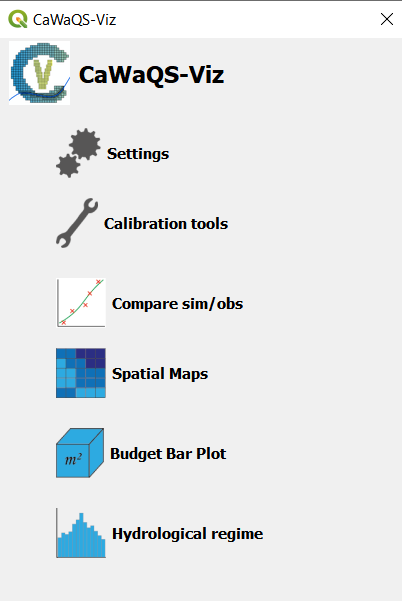
\includegraphics[width=0.4\linewidth]{
        2_application_user_guide/fig/CAWAQS_VIZ_home_page.png
    }
    \caption{Boîte de dialogue d'accueil de l'application \cwv.}
    \label{fig-cwv_home_page}
\end{figure}

\section{Configuration du plug-in \cwv}
\label{sec_config}

L'utilisation de l'extension \cwv~se fonde sur un projet \script{SIG} préexistant
contenant :
\begin{itemize}
    \item les maillages des différents modules de l'application \cawaqs, aux
        résolutions des sorties de modélisation ;

    \item les points d'observation et/ou les points d'extractions, situés dans les limites de l'emprise du modèle.
\end{itemize}

Le plug-in doit être configuré pour lire les différents fichiers de sortie de modélisation
et/ou d'entrée \cawaqs~ainsi que les différents maillages. Cette paramétrisation
du plug-in peut être effectuée dans la fenêtre \gui{Settings}. Pour ce faire, deux
procédures sont possibles :
\begin{itemize}
    \item importer un fichier de configuration \script{.json} préalablement
        établi ;

    \item configurer manuellement le projet dans la deuxième partie de la boîte de
        dialogue de la figure \ref{fig-DialogSettings}.
\end{itemize}

\begin{figure}[H]
    \centering
    % Première figure
    \begin{subfigure}
        [b]{0.45\linewidth}
        \centering
        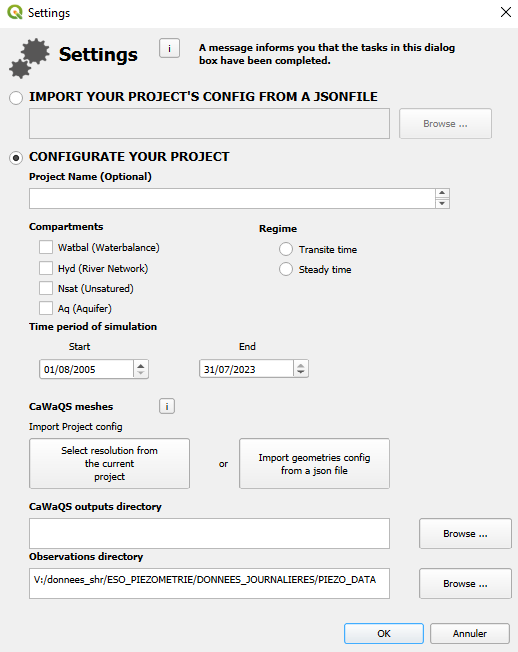
\includegraphics[width=\linewidth]{
            2_application_user_guide/fig/DialogSettings_creat_project.png
        }
        \caption{}
        \label{fig_DialogSettings_creat_projet}
    \end{subfigure}
    \hfill
    % Deuxième figure
    \begin{subfigure}
        [b]{0.45\linewidth}
        \centering
        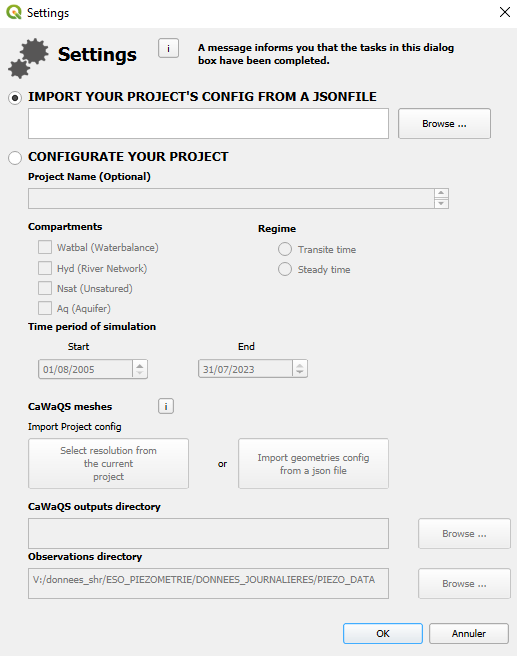
\includegraphics[width=\linewidth]{
            2_application_user_guide/fig/DialogSettings_import_project.png
        }
        \caption{}
        \label{fig_DialogSettings_inport_projet}
    \end{subfigure}
    \caption{Boîte de dialogue \gui{Settings} du plug-in. La méthode de
    configuration de l'application \cwv doit être sélectionnée : \textbf{(a)} création
    d'un nouveau projet \textbf{(b)} importation d'une configuration de projet. }
    \label{fig-DialogSettings}
\end{figure}

Les détails de ces deux procédures de configuration de l'application sont décrits
respectivement en paragraphes \ref{sec-config-manual} et \ref{sec-json_config_project}.

\section{Configuration manuelle du plug-in : première utilisation}
\label{sec-config-manual}

La partie inférieure de la boîte de dialogue \gui{Settings} permet de configurer
manuellement le plug-in. Les éléments suivants doivent y être définis :
\begin{enumerate}
    \item un nom de projet ;

    \item les compartiments modélisés ;

    \item une configuration des couches SIG des maillages ;

    \item les répertoires de sortie de modélisation et d'observation\footnote{les répertoires d'observation des débits et de piézométrie sont supposés être dans le même répertoire parent.} si des points d'observation sont définis dans le projet.
\end{enumerate}

Le nom du projet sera utilisé pour nommer un sous-dossier créé dans le répertoire
de post-traitement. Les sorties graphiques de l'application \cwv\ seront placées
dans ce dossier de post-traitement.\\

La configuration des géométries peut également être importée depuis un fichier de
configuration \json~(en cliquant sur \gui{Importer une configuration des géométries depuis un \json})
ou définie manuellement \textit{via} l'option \gui{Sélectionner les résolutions depuis le projet courant}.

\alertinfo{À noter que toute configuration manuelle de projet et de géométrie sera exportée au format \json~dans le répertoire de post-traitement à l'exécution de la boite de dialogue \gui{Settings}.}

\subsection{Contenu du projet QGIS utilisé pour l'exploitation des résultats de
simulations \cawaqs}
\label{sec-res-cawaqs}

\textbf{{Les \script{shapefiles} des maillages du modèle \cawaqs}}\\
Le projet QGIS utilisé pour le traitement des simulations avec l'utilitaire \cwv
nécessite de contenir :
\begin{itemize}
    \item les maillages (résolutions) des compartiments au format \gui{shapefile}
        du modèle (se référer à la notice \cawaqs~\footnote{Terminologie de
        géométrie \cawaqs. Pour plus d'informations sur les différents types de maillages,
        se référer aux notices du modèle (\ie~notice utilisateur et guide technique),
        disponibles sur le dépôt GitLab \href{https://gitlab.com/cawaqs/cawaqs}{https://gitlab.com/cawaqs/cawaqs}.}
        pour identifier les résolutions de sorties du compartiment \gui{WATBAL}).
        Les types de résolution \cawaqs~à importer dans le projet SIG en vue d'un
        traitement des sorties de modélisation sont fonction des compartiments
        effectivement modélisés ;

    \item les points d'observation des compartiments à définir dans l'extension \cwv.
\end{itemize}

\begin{table}[H]
    \centering
    \begin{tabular}{>{\raggedleft\arraybackslash}m{3cm}|>{\centering\arraybackslash}m{3.2cm}>{\centering\arraybackslash}m{3.2cm}>{\centering\arraybackslash}m{3.2cm}>{\centering\arraybackslash}m{3.2cm}}
        \hline
                                                                & \textbf{Compartiment de surface\newline(WATBAL)}                                                               & \textbf{Compartiment hydraulique \newline(HYD)} & \textbf{Compartiment non saturé \newline(NSAT)} & \textbf{Compartiment aquifère \newline(AQ)} \\
        \hline
        \textbf{Résolution \cawaqs}                             & Maille unitaire de surface (\texttt{ele\_bu})\footnotemark~ \newline ou Cellule de production (\texttt{Cprod}) & Élément rivière (\texttt{ele\_musk})            & Grille du milieu non saturé                     & Maillages de toutes les couches aquifères   \\
        \hline
        \textbf{Champs obligatoires dans la table attributaire} & Identifiants des cellules                                                                                      & Identifiants GIS des éléments rivières          & Identifiants des mailles                        & Identifiants absolus des mailles            \\
        \hline
    \end{tabular}
    \caption{Résolutions \cawaqs~pouvant être importées comme résolution de
    compartiment.}
    \label{tab-resolution_per_compartment}
\end{table}

\alertwarning{Les noms des couches SIG du projet correspondant aux aquifères doivent être identiques à ceux définis dans la configuration CaWaQS afin d'assurer le bon fonctionnement de l'application.}

\textbf{{Les \script{shapefiles} des points d'extractions}}\\

L'extraction des simulations de débit et de charge hydraulique peut être réalisée
aux droits de point d'extraction. Deux types types de points d'extraction peuvent être
renseignés :
\begin{itemize}
    \item des points d'extraction simple, qui n'intègrent pas de chronique de
        mesure ;

    \item des points d'observation, qui sont des points d'extraction avec des
        données de mesure.
\end{itemize}

Les points d'extraction et d'observation sont contenus dans deux fichiers
\script{shapefile} distinct dont les tables attributaires contiennent les champs
recensé dans la table \ref{tab_obs_extract}.

\vspace{8pt}

\renewcommand{\arraystretch}{1.5} % pour aérer les lignes
\newcolumntype{C}[1]{>{\centering\arraybackslash}p{#1}} \newcolumntype{C}[1]{>{\centering\arraybackslash}p{#1}}

\begin{table}[H]
    \begin{tabular}{|C{0.2\textwidth}|C{0.35\textwidth}|C{0.35\textwidth}|}
        \hline
        \textbf{TYPE DE POINT}& \textbf{CONTENUS DE LA TABLE ATTRIBUTAIRE} & \textbf{RENDUS} \tabularnewline                    \hline
        \textbf{Point d’extraction}  & 
        \begin{itemize}[leftmargin=*, itemsep=0.5ex]
            \item Nom du point
            \item Identifiant de la maille de rattachement\footnote{\gui{ID GIS} si extraction dans le compartiment HYD, \gui{ID ABS} si extraction en aquifère, champ optionnel}, identifiant de la couche aquifère (si extraction en aquifère)\end{itemize} & \begin{itemize}[leftmargin=*, itemsep=0.5ex]\item Hydrogrammes et courbes piézométriques simulés au droit du point d’extraction\end{itemize} \tabularnewline                     \hline
        \textbf{Point d’observation} & 
        \begin{itemize}[leftmargin=*, itemsep=0.5ex]
            \item Nom du point
            \item Identifiant de la maille de rattachement \footnotemark[\value{footnote}]
        \end{itemize} & 
        \begin{itemize}[leftmargin=*, itemsep=0.5ex]
            \item Hydrogrammes et courbes piézométriques simulés et observés
            \item Critères objectifs de comparaison entre les observations et les simulations
        \end{itemize} \tabularnewline \hline
    \end{tabular}
    \label{tab_obs_extract}
    \caption{Structure des couches SIG relatives aux points d’extraction et rendus graphiques associés}
\end{table}

\vspace{8pt}

\alertwarning{Les \script{shapefile} d'observation doivent être importée dans le projet et renseignée dans la configuration de \cwv~si les compartiements HYD et/ou AQ sont traités. Sans observations l'extention ne sera pas fonctionnelle}

\subsection{Configuration de la géométrie du projet depuis un projet QGIS
existant}
\label{sec_config_manuelle}

La configuration géométrique de l'application \cwv peut être définie depuis un projet
QGIS existant via la boite de dialogue \gui{Application configuration from an existing projet}
de la boite de dialogue de paramétrage de l'application.

La fenêtre est organisée selon deux sections :
\begin{itemize}
    \item sur la gauche, sont listés les compartiments \cawaqs (WATBAL, HYD, AQ,
        NSAT),

    \item sur la droit, sont listé les paramètres à définir pour produire les
        rendus graphique (débit et piézométrie) aux droits de points d'observation
        (point d'extraction avec observation) ou de points d'exctration (sans observation).
\end{itemize}

Si les champs de paramétrage de l'application sont laissé vide, le compartiment
concerné n'est pas intégrer dans la configuration géométrique. \\

Les champs des compartiments sont configurés suivant :\\

\noindent
\textbf{Le compartiment de surface (\gui{"WATBAL COMPARTMENT"}) :}

\vspace{0.5em}

\begin{minipage}[t]{0.45\textwidth}
    \begin{itemize}
        \item \gui{Surface resolution} : résolution de sortie du bilan hydrique de surface (CPROD ou elebu) ;
        \item \gui{cell id} : le numéro de la colonne dans la table attributaire qui correspond à l'identifiant des mailles ;
        \item \gui{cell area} : le numéro de la colonne dans la table attributaire qui correspond à la surface des mailles (paramètre optionnel).
    \end{itemize}
\end{minipage}%
\hfill
\begin{minipage}[t]{0.45\textwidth}
    \centering
    \raisebox{\dimexpr-\height+\ht\strutbox}{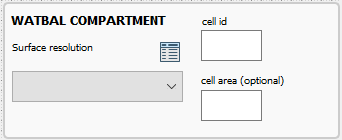
\includegraphics[
        width=0.8\linewidth
    ]{
        2_application_user_guide/fig/DialogSelectLayer_watbal.png
    }} \captionof{figure}{Champ de paramétrage du compartiment WATBAL}
\end{minipage}

\vspace{1em}
\textbf{Le compartiment hydrologique (\gui{HYD COMPARTMENT})}

\begin{minipage}[t]{0.45\textwidth}
    \begin{itemize}
        \item \gui{Hyd resolution} : nom de la résolution de sortie du compartiment \gui{HYD} (éléments rivières) ;
        \item \gui{GIS Id} : le numéro de la colonne dans la table attributaire qui correspond à l'identifiant GIS des mailles 
    \end{itemize}
\end{minipage}%
\hfill
\begin{minipage}[t]{0.45\textwidth}
    \centering
    \raisebox{\dimexpr-\height+\ht\strutbox}{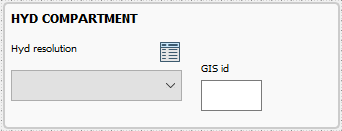
\includegraphics[
        width=0.8\linewidth
    ]{
    2_application_user_guide/fig/DialogSelectLayer_hyd.png
    }} 
    \captionof{figure}{Champ de paramétrage du compartiment HYD}
\end{minipage}

\vspace{1em}
\textbf{Le compartiment non saturé (\gui{NSAT COMPARTMENT}):}

\begin{minipage}[t]{0.45\textwidth}
    \begin{itemize}
        \item \gui{Unsatured zone resolution} : nom de la résolution de sortie du compartiment \gui{NSAT} ;
        \item \gui{cell id} : le numéro de la colonne dans la table attributaire qui correspond à l'identifiant des mailles. 
    \end{itemize}
\end{minipage}%
\hfill
\begin{minipage}[t]{0.45\textwidth}
    \centering
    \raisebox{\dimexpr-\height+\ht\strutbox}{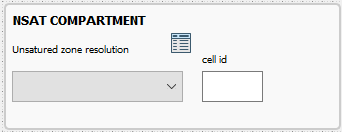
\includegraphics[
        width=0.8\linewidth
    ]{
    2_application_user_guide/fig/DialogSelectLayer_nsat.png
    }} 
    \captionof{figure}{Champ de paramétrage du compartiment HYD}
\end{minipage}

\vspace{1em}
\textbf{Le compartiment saturé (\gui{AQ COMPARTMENT})}

\begin{minipage}[t]{0.45\textwidth}
     \begin{itemize}
            \item \gui{Aquiferes resolutions} : les couches SIG constituant le
                maillage souterrain. La couche sélectionnée est ajoutée en cliquant
                sur \gui{Add}. Les couches doivent être ordonnées de la couche supérieure
                à la couche inférieure à l'aide des boutons \gui{up} et \gui{down}.
                Enfin, une couche peut être supprimée de la liste en cliquant sur
                \gui{remove} ;
            \item \gui{cell id abs} : identifiant de la colonne de la table
                attributaire contenant l'identifiant absolu des mailles. Cet identifiant
                peut être homogène entre les couches SIG : dans ce cas, \gui{homogeneous ID ABS}
                doit être sélectionné. Sinon, cliquer sur \gui{heterogeneous ID ABS}
                pour ouvrir des boîtes de dialogue permettant de renseigner, pour
                chaque couche, la colonne contenant l'ID ABS des mailles (cf. Fig \ref{fig_id_abs_hetero}).
        \end{itemize}
\end{minipage}%
\hfill
\begin{minipage}[t]{0.45\textwidth}
    \centering
    \raisebox{\dimexpr-\height+\ht\strutbox}{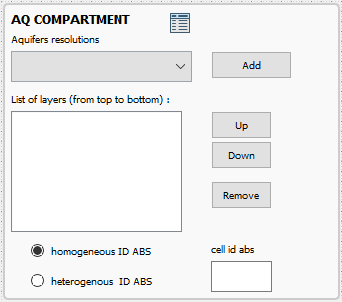
\includegraphics[
        width=0.8\linewidth
    ]{
    2_application_user_guide/fig/DialogSelectLayer_aq.png
    }} 
    \captionof{figure}{Champ de paramétrage du compartiment HYD}
    \raisebox{\dimexpr-\height+\ht\strutbox}{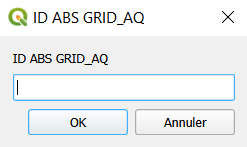
\includegraphics[
        width=0.5\linewidth
    ]{
2_application_user_guide/fig/DialogSelect_Layer_hetero_ID_ABS
    }} 
    \label{fig_id_abs_hetero}
    \captionof{figure}{Fenêtre de sélection de l'identifiant du champ contenant l'\gui{ID ABS} dans la table attributaire dans le cas d'identifiant de champ hétérogène entre les couches}
\end{minipage}



\alertwarning{Quelques point de vigilance :
\begin{itemize}
    \item \textbf{L'identifiant de la première colonne d'une table attributaire commence à 0}. L'icône 
\includegraphics[height=0.45cm]{2_application_user_guide/fig/table.png} permet de visualiser les identifiants des champs renseignés dans la table attributaire de la résolution sélectionnée dans la liste déroulante ;
    \item le code (ex : code BSS) d'un point d'observation doit être \textbf{unique} entre tous les points d'observation ;
    \item La configuration géométrique des compartiments cochés dans la boite de dialogue de paramétrisation du projet, doit être définie dans la boite de dialogue de configuration des géométries.
\end{itemize}}

\vspace{8pt}

\textbf{Les points d'extraction - \gui{Hydrological and Hydrological plots}} \\
Les points d'extraction peuvent être de deux types :
\begin{itemize}
    \item[$\bullet$] des points d'extractions simples, qui permettent de
    visualiser des variables simulées au droit d'un point de ces derniers ;
    \item[$\bullet$] des points d'observation, qui permettent de comparer les variables simulées à des données d'observation aux droits de ces derniers.
\end{itemize}



La configuration des points d'extraction nécessite de renseigner dans les champs \gui{GIS Layer}, la nom de la couche dans le projet QGIS contenant les points d'observations et les points d'extraction selon le compartiment \cws~ concerné. Les identifiants des champs à renseigner sont les suivants : 
\vspace{8pt}

\begin{minipage}[t]{0.45\textwidth}
    \textbf{Les points d'extraction du compartiment \gui{HYD}} 
    \vspace{4pt}

     \underline{Les points d'extraction}

    \begin{itemize}
        \item \gui{name} : nom du point d'observation ;
        \item \gui{ID GIS} : identifiant GIS du point d'observation auquel le point d'observation doit être attaché (champ optionnel)
    \end{itemize}

    \vspace{2pt}
    \underline{Les points d'observation} 
    \begin{itemize}
        \item \gui{code} : code d’identification du points d'observation, doit être un code unique pour chaque point. Le fichier d'observation du point doit porte le même nom sous l’extension \script{.dat} ;
        \item les champ \gui{name} et \gui{ID GIS} sont également préciser pour la configuration des points d'observation 
    \end{itemize}
    \vspace{8pt}
    \textbf{Les points d'extraction du compartiment \gui{AQ}} 
    \vspace{4pt}

     \underline{Les points d'extraction}

    \begin{itemize}
        \item \gui{name} : nom du point d'observation ;
        \item \gui{ID LAYER} : identifiant de la couche aquifère
        \item \gui{ID GIS} : identifiant GIS du point d'observation auquel le point d'observation doit être attaché (champ optionnel)
    \end{itemize}

    \vspace{2pt}
    \underline{Les points d'observation} 
    \begin{itemize}
        \item \gui{code} : code d’identification du points d'observation, doit être un code unique pour chaque point. Le fichier d'observation du point doit porté le même nom sous l’extension \script{.dat} ;
        \item les champ \gui{name} et \gui{ID GIS} sont également préciser pour la configuration des points d'observation 
    \end{itemize}

    
\end{minipage}%
\hfill
\begin{minipage}[t]{0.45\textwidth}
    \centering
    \raisebox{\dimexpr-\height+\ht\strutbox}{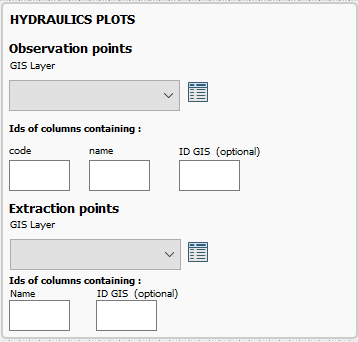
\includegraphics[
        width=0.9\linewidth
    ]{
    2_application_user_guide/fig/DialogSelectLayer_hyd_extraction.png
    }} 
    \captionof{figure}{Champs de configuration des points d'extraction du compartiment \gui{HYD}}
    \vspace{4pt}
    \raisebox{\dimexpr-\height+\ht\strutbox}{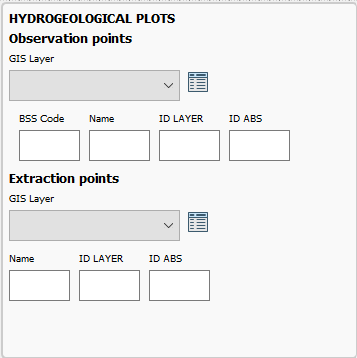
\includegraphics[
        width=0.9\linewidth
    ]{
    2_application_user_guide/fig/DialogSelectLayer_aq_extraction
    }} 
    \label{fig_id_abs_hetero}
    \captionof{figure}{Champs de configuration des points d'extraction du compartiment \gui{AQ}}
\end{minipage}

\alertwarning{
Le points d'extraction doivent être contenus dans un fichier \script{.shp} différent des points d'observtion. Les points ne peuvent pas être contenu dans le même fichier s'il s'agit d'extraction dans deux compartiment différent.
}


\alertinfo{
Une sauvegarde préliminaire du fichier de configuration géométrique peut être sauvegardé en renseignant un chemin de fichier dans le champ situé en bas à gauche de la boite de dialogue. Ce fichier (\cfcod \ref{code_config_geom})  sera enregistré à l'exucution de la boite de dialogue \gui{Settings} si le  si le projet configuré n'existe pas encore dans le répertoire
de post-traitement renseigné. 
Plusieurs configurations de projet peuvent être sauvegardées dans un même répertoire de post-Processing, sous réserve qu'elles n'aient
pas le même nom de projet. }



\subsection{Configuration des résolutions depuis un fichier de configuration
\json}

La configuration géométrique des résolutions peut être renseignée par un fichier
\json\ selon la structure suivante :

\begin{lstlisting}[language=json, caption={Contenu d'un fichier de configuration géométrique}, label={code_config_geom}]
{   // liste des compartiments CaWaQS a analyser (1 = AQ, 2 = HYD, 3 = WATBAL) 
    "ids_compartment": [], 
                           
    "resolutionNames": 
    {
        "1": 
            [[""]], // liste des noms des maillages aquiferes dans le projet QGIS 
        "2" : 
            [[""]], // liste du nom du maillages riviere dans le projet QGIS 
        "3" : 
            [[""]] // liste du nom du maillage de surface dans le projet QGIS 
        "4" : 
            [[""]] // liste du nom du maillage du non-sature dans le projet QGIS 
        }, 
    "ids_col_cell": { // "id compartiment" : "no de la colonne de l'id des mailles"
        "1" : "",  // "id AQ" : "no de la colonne de l'id absolue"
        "2" : "",  //"id HYD" : "no de la colonne de l'id GIS"
        "3" : ""   // "id WATBAL" : "no de la colonne de l'id de la maille"
        }, 
    "obsNames": { 
    // "id compartiment" : "nom du shp des obs associes dans le projet QGIS"
        "1": "", 
        "2" : ""
        }, 
    "obsIdsColCells": {
    // "id compartiment" : "no du champ du code du point de mesure"
        "1": "", 
        "2": ""
        }, 
    "obsIdsColNames": { 
    // "id compartiment" : "no du champ du nom du point de mesure"
        "1": "", 
        "2" : ""
        }, 
    "obsIdsColLayers": { 
    // "id compartiment" : "no du champ de l'identifiant de la couche aquifere"
        "1": "", 
        "2" : null
        }, 
    "obsIdsCell": { 
    // "id comp." : "no du champ de l'id absolu ou gis de maille ratachee a l'obs
        "1" : "", 
        "2" : null
    }, 
     "extNames": {
    // "id compartiment" : " nom du shp d'extraction associes dans le projet QGIS "
        "2": "",
        "1": ""
    },
    "extIdsColNames": {
    // "id compartiment" : "no du champ contenant le nom du point d'extraction"
        "2": "",
        "1": ""
    },
    "extIdsColLayers": {
    // "id compartiment" : "no du champ contenant l'identifiant de la couche aquifere"
        "2": null,
        "1": ""
    },
    "extIdsColCells": {
    // "id compartiment" : "no du champ contenant l'identifiant de la maille"
        "1": "",
        "2": "",
    }
}
}
\end{lstlisting}

\subsection{Contenu du répertoire de post-traitement}

À l'exécution de la boîte de dialogue de paramétrage de l'application \cwv, le
sous-répertoire du projet est créé dans le répertoire de post-traitement indiqué.
Si le projet n'existe pas encore dans ce répertoire, un sous-répertoire au nom
du projet sera créé, contenant les fichiers de configuration du projet et des résolutions,
écrits au format \gui{json}.

\section{Configuration du projet depuis un fichier de configuration projet \json}
\label{sec-json_config_project}

L'import d'un fichier externe \json~peut également être utilisé pour configurer
du projet. Ce fichier est construit de la manière suivante

\begin{lstlisting}[language=json]
{
    "json_path_geometries": str,
    "projectName": str, 
    "cawOutDirectory": str,
    "startSim": int,
    "endSim": int,
    "obsDirectory": str,
    "ppDirectory": str, 
    "regime": str
}
\end{lstlisting}

\vspace{-0.6cm}
Le contenu de chaque objet de ce fichier \json~est le suivant :
\begin{itemize}
    \item \gui{json\_path\_geometries} : chemin absolu du fichier de
        configuration des résolutions ;

    \item \gui{projectName} : nom du projet ;

    \item \gui{cawOutDirectory} : chemin absolu du répertoire contenant les
        sorties de modélisation \cawaqs~;

    \item \gui{startSim} et \gui{endSim} : années de départ et de fin de la simulation
        au format \script{integer} ;

    \item \gui{obsDirectory} : chemin absolu du répertoire parent contenant les
        chroniques observées ;

    \item \gui{ppDirectory} : chemin absolu du répertoire de post-traitement. Il
        est à noter que le chemin doit être pré-existant. Le cas échéant, il ne sera
        pas créé par l'application.

    \item \gui{regime} : régime de modélisation ("Transient" ou "Steady")
\end{itemize}